\section{Chandra Kirana Poetra (1174079)}
\subsection{Menggunakan LeafletJS dengan MapProxy}
\begin{enumerate}
    \item Jalankan dulu mapproxy yang kemarin telah dibuat di gede-master
    \hfill\break
    \begin{figure}[H]
		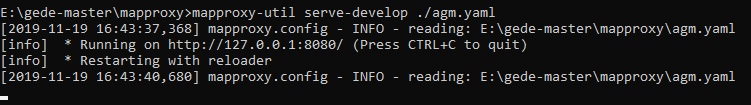
\includegraphics[width=12cm]{figures/Tugas5/1174079/1.png}
		\centering
		\caption{Gambar 1}
	\end{figure}
    \item Buka file basic.html di folder LeafletJS di dalam folder gede
    \hfill\break
    \begin{figure}[H]
		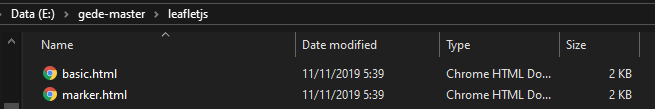
\includegraphics[width=12cm]{figures/Tugas5/1174079/2.png}
		\centering
		\caption{Gambar 2}
	\end{figure}
    \item Berikut adalah hasil dari file basic.html
    \hfill\break
    \begin{figure}[H]
		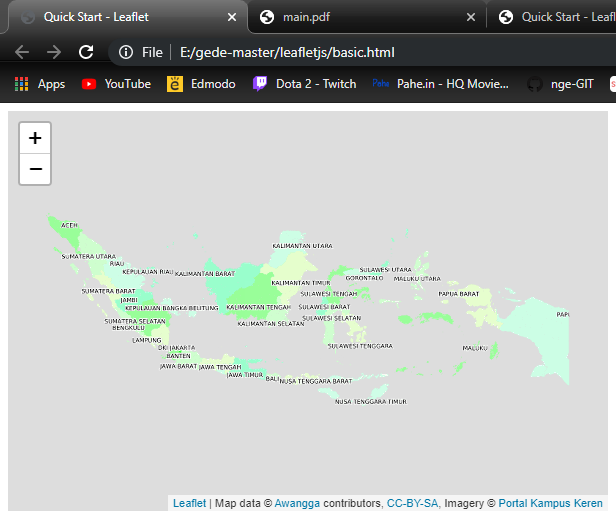
\includegraphics[width=12cm]{figures/Tugas5/1174079/3.png}
		\centering
		\caption{Gambar 3}
	\end{figure}
    \item Di leafletjs kita juga bisa menambahkan penanda atau marker,circle, ataupun polygon sebagai penanda dengan cara seperti di gambar
    \hfill\break
    \begin{figure}[H]
		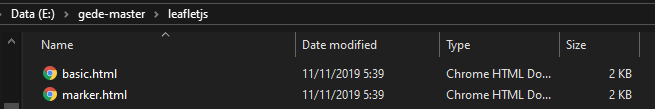
\includegraphics[width=12cm]{figures/Tugas5/1174079/2.png}
		\centering
		\caption{Gambar 4}
	\end{figure}
	\begin{figure}[H]
		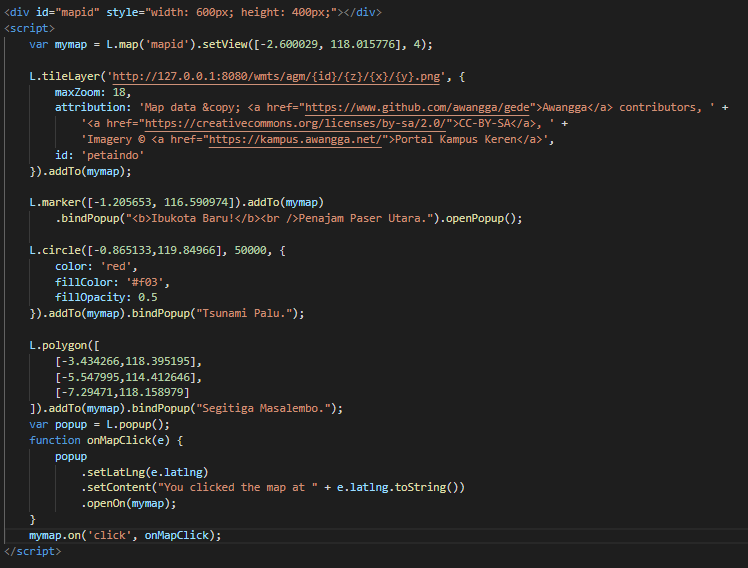
\includegraphics[width=12cm]{figures/Tugas5/1174079/4.png}
		\centering
		\caption{Gambar 5}
	\end{figure}
    \item Lalu coba buka di browser
    \hfill\break
    \begin{figure}[H]
		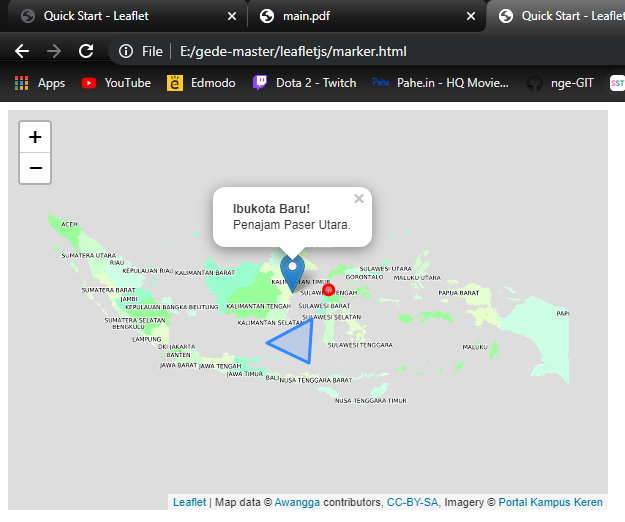
\includegraphics[width=12cm]{figures/Tugas5/1174079/5.png}
		\centering
		\caption{Gambar 6}
	\end{figure}
\end{enumerate}
\subsection{Link Youtube}
https://youtu.be/0PGjQqv-Dec